\documentclass{beamer}
\usetheme{Warsaw}

\usepackage{amsfonts} % math symobls
\usepackage{amsthm}
\usepackage[utf8]{inputenc}
\usepackage{polski}
\usepackage{graphics}
\usepackage{verbatim}

\newcommand{\emp}[1]{\textcolor{blue}{\textit{#1}}}
\newcommand{\red}[1]{\textcolor{red}{#1}}

\title{Rozpoznawanie chorób skóry}
\author{Michał Karpiński}
\date{24 stycznia, 2013}

\begin{document}

\begin{frame}[plain]
  \titlepage
\end{frame}

\begin{frame}{Choroby skóry}

\begin{columns}
\begin{column}{0.5\textwidth}
\begin{center}
  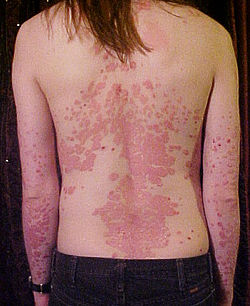
\includegraphics[scale=0.5]{img/psoriasis.jpg}

  Łuszczyca
\end{center}
\end{column}
\begin{column}{0.5\textwidth}
\begin{center}
  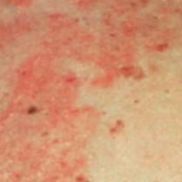
\includegraphics[scale=0.5]{img/seboreic_dermatitis.jpeg}  

  Łojotokowe zapalenie skóry
\end{center}
\end{column}
\end{columns}
\end{frame}

\begin{frame}{Choroby skóry}

\begin{columns}
\begin{column}{0.5\textwidth}
\begin{center}
  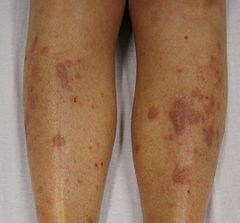
\includegraphics[scale=1.5]{img/lichen_planus.jpg}

  Liszaj płaski
\end{center}
\end{column}
\begin{column}{0.5\textwidth}
\begin{center}
  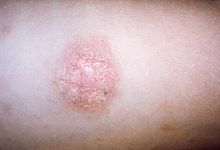
\includegraphics[scale=1.5]{img/pityriasis_rosea.jpg}  

  Łupież różowy Giberta
\end{center}
\end{column}
\end{columns}
\end{frame}

\begin{frame}{Choroby skóry}

\begin{columns}
\begin{column}{0.5\textwidth}
\begin{center}
  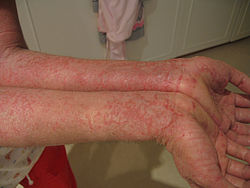
\includegraphics[scale=0.7]{img/chronic_dermatitis.jpg}

  Atopowe zapalenie skóry
\end{center}
\end{column}
\begin{column}{0.5\textwidth}
\begin{center}
  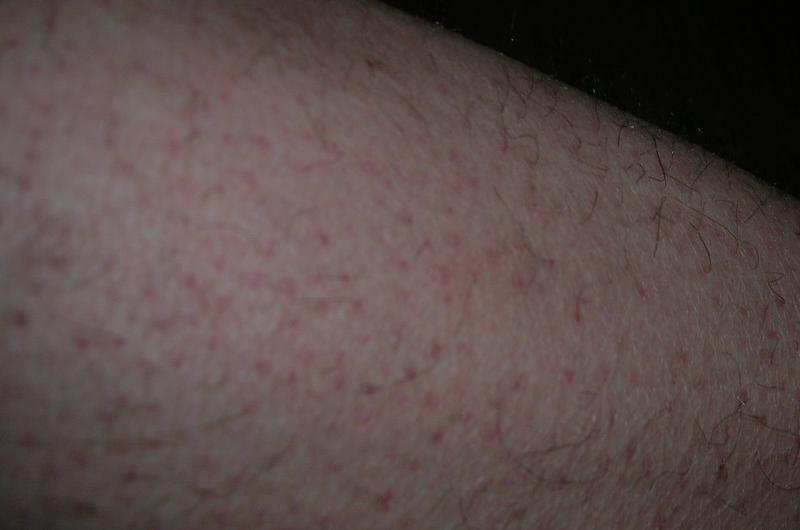
\includegraphics[scale=0.2]{img/pityriasis_rubra_pilaris.jpg}  

  Rogowacenie przymieszkowe czerwone
\end{center}
\end{column}
\end{columns}
\end{frame}

\begin{frame}{Dane}
\begin{block}{Źródło}
{\em http://archive.ics.uci.edu/ml/datasets/Dermatology}
\end{block}

\begin{itemize}
\item Liczba próbek: 366
\item Liczba cech: 34
\item Liczba klas: 6
\end{itemize}

\end{frame}

\begin{frame}{Dane - liczba osobników w danej klasie}

\begin{center}
  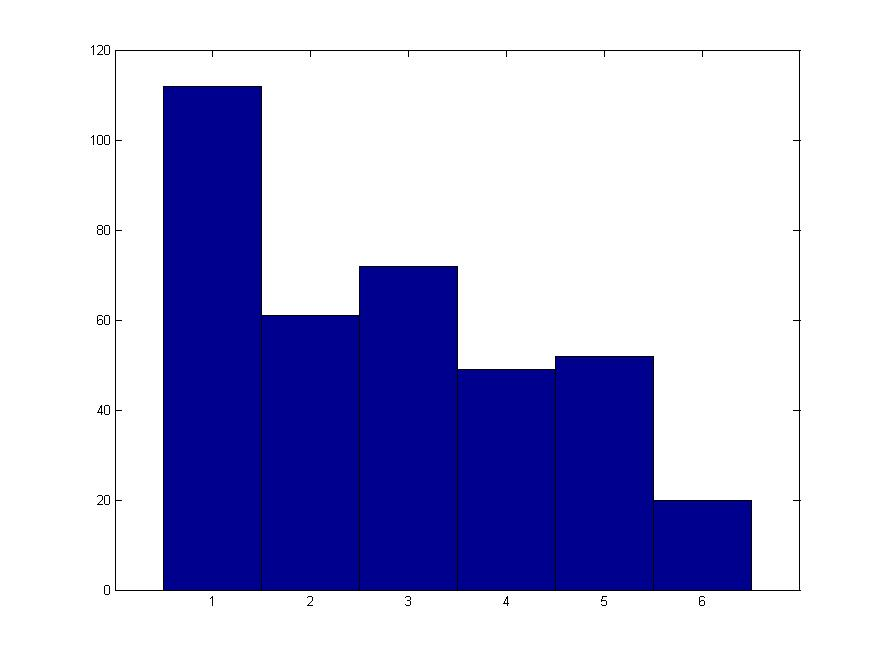
\includegraphics[scale=0.35]{img/class_hist.jpg}  
\end{center}

\end{frame}

\begin{frame}{Dane - cechy kliniczne}
  \begin{itemize}
    \item zaczerwienienie
    \item skala zmian
    \item swędzenie
    \item kształt
    \item miejsce występowania
    \item wiek
    \item występowanie choroby w rodzinie
  \end{itemize}
\end{frame}

\begin{frame}{Dane - cechy histopatologiczne}
\begin{itemize}
\item PNL infiltrate
\item exocytosis
\item acanthosis
\item hyperkeratosis
\item parakeratosis
\item clubbing of the rete ridges
\item elongation of the rete ridges
\item thinning of the suprapapillary epidermis
\item spongiform pustule
\item munro microabcess
\item focal hypergranulosis
\item spongiosis
\item saw-tooth appearance of retes
\item follicular horn plug
\item perifollicular parakeratosis
\item band-like infiltrate
\end{itemize}
\end{frame}

\begin{frame}{Dane - dziedzina cech}
Wartości wszystkich cech zmierzone zostały w czterostopniowej skali \{0,1,2,3\}.

\vspace{0.5cm}

Wyjątki:
\begin{itemize}
\item występowanie choroby w rodzinie - \{0,3\}
\item wiek - liczba naturalna
\end{itemize}

\end{frame}

%       1             psoriasis(łuszczyca)	     112
%       2             seboreic dermatitis(łojotokowe zapalenie skóry)             61
%       3             lichen planus(liszaj płaski)    72
%       4             pityriasis rosea (łupież różowy Giberta)                49
%       5             chronic dermatitis (atopowe zapalenie skóry)               52    
%       6             pityriasis rubra pilaris (Rogowacenie przymieszkowe czerwone)       20
%
% Clinical Attributes: (take values 0, 1, 2, 3, unless otherwise indicated)
%      1: erythema
%      2: scaling
%      3: definite borders
%      4: itching
%      5: koebner phenomenon
%      6: polygonal papules
%      7: follicular papules
%      8: oral mucosal involvement
%      9: knee and elbow involvement
%     10: scalp involvement
%     11: family history, (0 or 1)
%     34: Age (linear)
%
% Histopathological Attributes: (take values 0, 1, 2, 3)
%     12: melanin incontinence
%     13: eosinophils in the infiltrate
%     14: PNL infiltrate
%     15: fibrosis of the papillary dermis
%     16: exocytosis
%     17: acanthosis
%     18: hyperkeratosis
%     19: parakeratosis
%     20: clubbing of the rete ridges
%     21: elongation of the rete ridges
%     22: thinning of the suprapapillary epidermis
%     23: spongiform pustule
%     24: munro microabcess
%     25: focal hypergranulosis
%     26: disappearance of the granular layer
%     27: vacuolisation and damage of basal layer
%     28: spongiosis
%     29: saw-tooth appearance of retes
%     30: follicular horn plug
%     31: perifollicular parakeratosis
%     32: inflammatory monoluclear inflitrate
%     33: band-like infiltrate

\end{document}
